% Generated by scripts/lecture09_interpolants.py; edit the generator.
\begin{figure}[htbp]
\centering
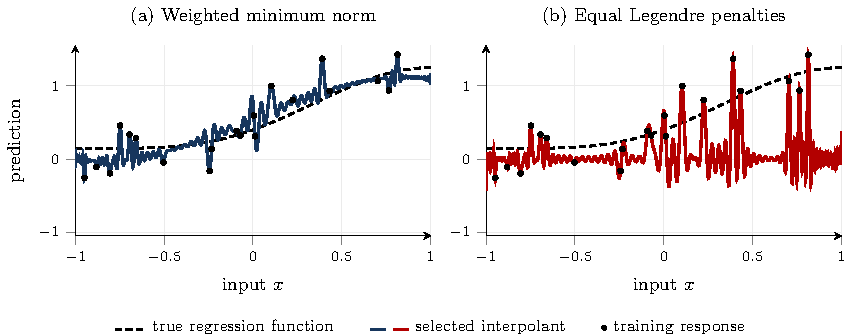
\includegraphics[width=\linewidth]{../figures/lecture09-polynomial-interpolants-plot.pdf}
\caption{Both panels use the same $n=20$ observations from
$X\sim\operatorname{Unif}[-1,1]$ and
$Y=f^\star(X)+\cN(0,0.28^2)$, where
$f^\star(x)=0.55+0.55\sin(\pi x/2)-0.15\cos(\pi x)$, and the same space of
dimension $164$. Both rules interpolate. The weighted norm distinguishes
the first $m=4$ features; equal Legendre penalties minimize $L^2(\mu)$ norm.}
\label{fig:polynomial-interpolants}
\end{figure}
